%
% $Id: ch04_implementation.tex
%
%   *******************************************************************
%   * SEE THE MAIN FILE "AllegThesis.tex" FOR MORE INFORMATION.       *
%   *******************************************************************
%
\chapter{Results and Evaluation}\label{ch:reseval}
Following the implementation specifications set forth in the previous chapters, a functional image sharing website was developed. This website was not only able to successfully accept images, store them for later access, and provide these features in an intuitive manner, but it did so while reducing its storage space requirements. In order to gauge the success of the research project, several metrics must be evaluated. The first to be considered is the functionality of the image sharing system. This includes usability and the requirement of keeping user interaction at a minimum while the space optimization system operates behind the scenes. Along with functionality, the performance of the system must be evaluated. If the addition of the developed system takes too much time to operate, a user might be dissuaded from using the system in the first place. This would in fact lessen storage requirements of the image sharing website, but defeats the purpose of the research. Performance has been measured in in several ways, namely the processing time to upload an image to the server, accuracy of duplicate detection, and the amount of storage space required after duplicate detection has run. As this research hinges on the performance of the duplicate detection algorithm from a time and effectiveness standpoint, the results are of extreme importance. This chapter presents the results of the system's evaluation against the characteristics outlined above.

\section{Functionality}
As mentioned previously, the functionality of the image sharing website developed involves both the usability and autonomous function of the server side duplicate detection system. In order to gain insight into the usability of the image sharing system, one must first understand how it is operated. Upon loading of the web page the user is presented with a screen as shown in Figure \ref{fig:shareprompt}.

At this time, the user is asked to select an image for sharing and is told that only jpeg images are allowed. This can be accomplished by using the given option to browse for an image file stored on their local computer. Upon choosing an allowed image, a preview will be displayed along with the details of the image to be uploaded.

If a user would choose to upload a file that is not of the jpeg format or if the image size is larger than what the server allows, a warning will be displayed and the upload button will remain disabled as seen in Figures \ref{fig:typewarning} and \ref{fig:sizewarning}.

\begin{figure}[htbp]
\centering
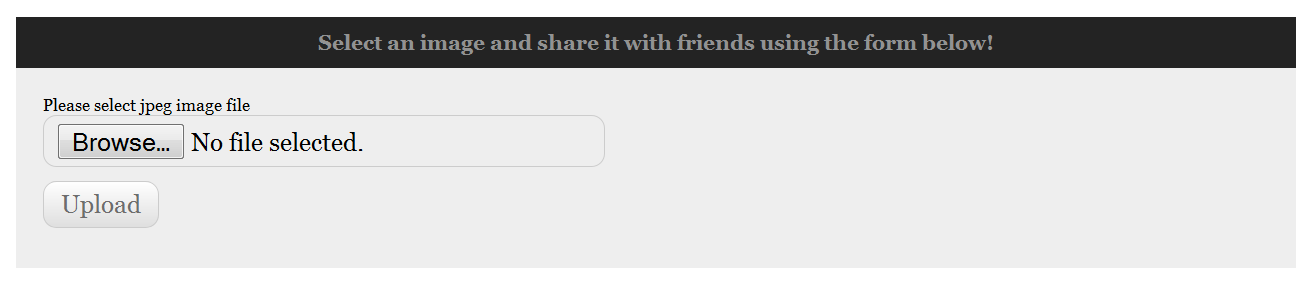
\includegraphics[width=6in]{uploadform}
\caption{Initial state of the upload form upon page load.}
\label{fig:shareprompt}
\end{figure}

\begin{figure}[htbp]
\centering
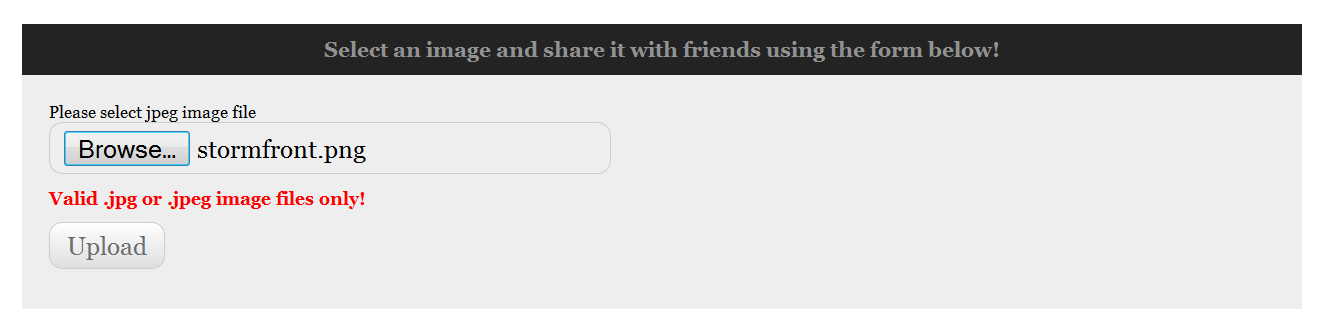
\includegraphics[width=6in]{typewarning}
\caption{Error displayed when a user attempts to upload a non-jpeg file.}
\label{fig:typewarning}
\end{figure}

\begin{figure}[htbp]
\centering
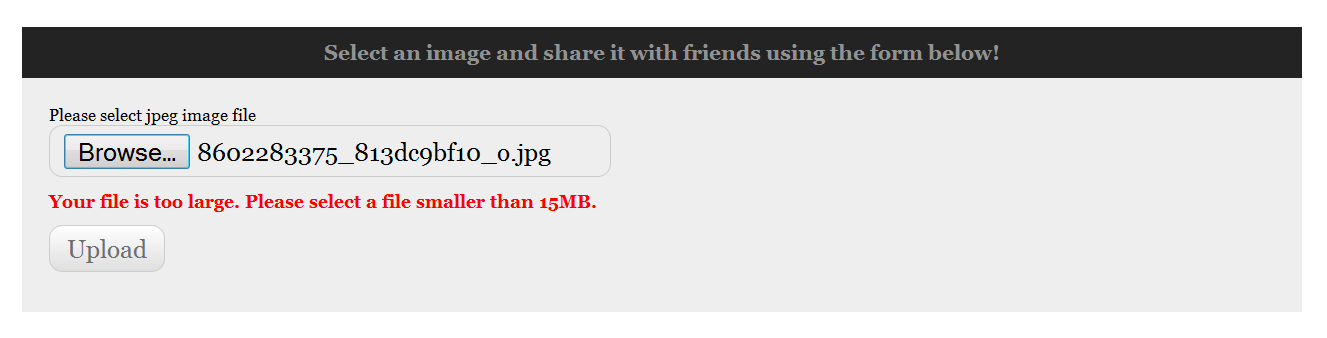
\includegraphics[width=6in]{sizewarning}
\caption{Error displayed when attempting to upload a jpeg image that is too large.}
\label{fig:sizewarning}
\end{figure}

By designing the system in this manner, it ensures that the image upload can be completed in an intuitive way. After any errors have been resolved by selecting an appropriate sized jpeg file, the upload button will enable and the user can click it to start the sharing process. Once the upload begins a new section of the user interface will be built and displayed. In this section, a progress bar is visible that visualizes the current progress of the image transfer to the server, the speed in which the transfer is occurring, and the estimated time remaining. Upon completion of the upload, the user is presented with a message saying "PLEASE WAIT...PROCESSING", which can be seen in figure \ref{fig:imageprocessing}. During this time, the algorithms operate in the background determining the images uniqueness as implemented in Chapter \ref{ch:method}. To this point, the only interaction required by the user is supplying an acceptable image file and clicking the upload button. After processing completes, there are several options that can be displayed.

\begin{figure}[htbp]
\centering
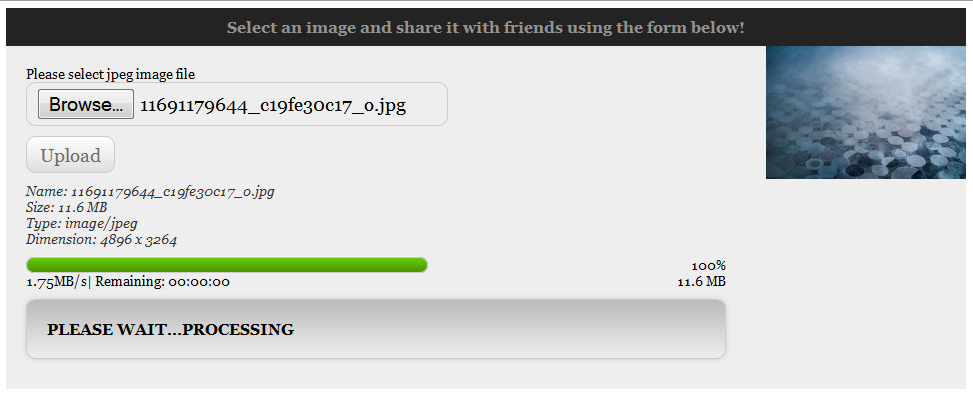
\includegraphics[width=6in]{imageprocessing}
\caption{Image processing after upload completes.}
\label{fig:imageprocessing}
\end{figure}

If it is determined that the image being uploaded is a potential duplicate, a pop-up is displayed to the user with a preview of the image they are trying to upload shown side by side with a preview of the potential duplicate on the server. The image with a higher resolution has text displayed under it specifying. The user can then click the higher resolution image and the server will provide the link to share it with, or they can choose to upload their image anyway. At this point, the server assumes the image is unique and will generate and display a link to the user. This feature was disabled for the purpose of testing the effectiveness as it introduces a human error which could bias collected results. If the image is in fact deemed to be unique, user interaction is not required. The server will generate a link to the new image and return it to the user for sharing.

From this point on, the full upload process is complete, and users can access an image using one of the generated links, never knowing if that image was unique or is displaying the copy already on the server. Although this system is very basic on the surface, it is very powerful. Not only is the server reducing image duplication in real time, but it is simultaneously generating links, thumbnails and possibly performing other uploads and serving images to users all with the click of two buttons or one link.

\section{Performance}
Processing time in the scope of this research refers to the amount of real world time that it takes to complete the image upload. This begins at the point where the server receives an image to the time where a link is provided to the user. As seen in Figures \ref{fig:proctimenodup} and \ref{fig:proctimemixdup}, several factors play a major role in the variance of processing time.

\begin{figure}[htbp]
\centering
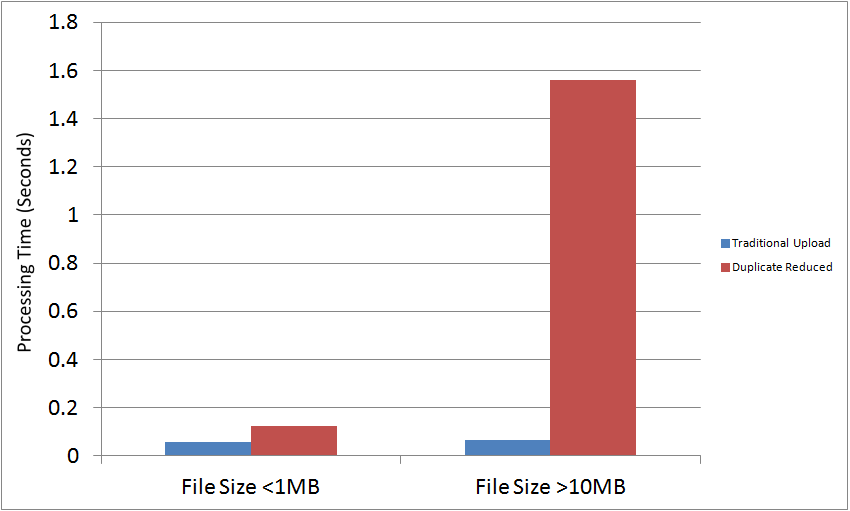
\includegraphics[width=4in]{proctimenodup}
\caption{Processing time on data set without duplicates.}
\label{fig:proctimenodup}
\end{figure}

\begin{figure}[htbp]
\centering
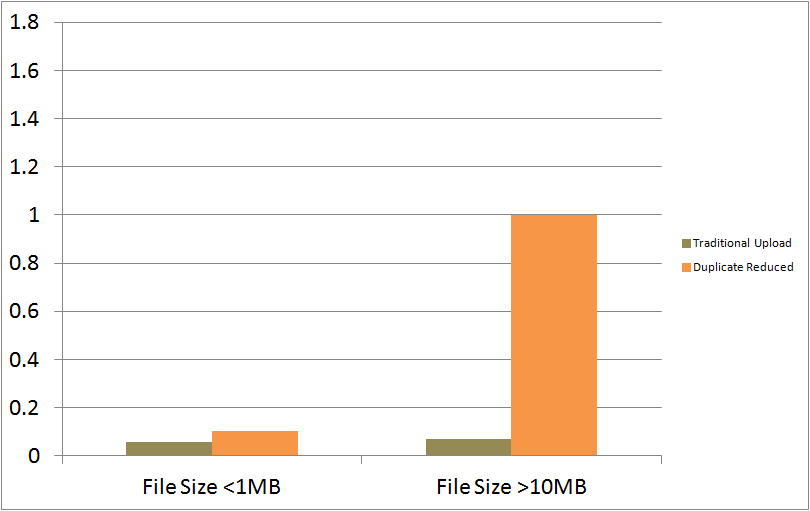
\includegraphics[width=4in]{proctimemixdup}
\caption{Processing time on data set with 20\% duplicate images.}
\label{fig:proctimemixdup}
\end{figure}

Of any variable tested, file size was determined to have the largest impact on processing time. Although at first glance, the large image upload using this system may appear too inefficient for a real world scenario, it is important to remember the scale being used. Traditional upload methods appeared almost instantaneous to the user while duplicate reduced took less than two seconds to process, even on the largest file. This amount of time was not considered unreasonable as fluctuations in Internet connection speed can cause greater variance in upload times than was ever observed with processing times from the server side. To interpret the graphs in an intuitive manner, it can be said that processing time is directly proportional to the size of the files being uploaded. In addition, the average processing time can be greatly affected by the frequency of duplicates being uploaded. When exact duplicates are uploaded the processing time is near that of a traditional upload as the in-depth image scan is not needed. This fact alone can account for another large source of processing time variance. In Figure \ref{fig:proctimenodup}, every file was chosen to be unique, this would cause data to be collected that reflected worst case processing time where every file was scanned in depth. In Figure \ref{fig:proctimemixdup}, a data set was created that contained 20\% exact duplicate images. This number was chosen as it correlated to the estimated amount of duplicate data on servers which is discussed previously in Section \ref{sec:motivation}. In this case a smaller number of images required a detailed analysis, while the remaining images were able to be detected with only a first pass scan. In this scenario, the processing time was reduced by approximately 30\% of the worst case time.

Although these results point toward a feasible system with respect to wait time, server configuration and load can affect these greatly. A webmaster can decide to accept larger or smaller images than the 15MB limit that was configured for this experiment. Seeing that processing times increase rapidly with respect to file size, this system leans toward a usage on high volume servers with a smaller image size versus a low volume situation with large files.

Next, another important metric is the total space consumption of the images uploaded. Using four test sets of images the results were compiled and quite promising. The first test set included images smaller than 1MB with no duplicates included. As expected, this set required the same amount of space after duplicate reduction as a traditional upload system. The same could be said for the other group of large images with no duplicates. In the group containing small images with one of five chosen modifications including 85\% quality reduction, 25\% resolution reduction, horizontal flip, vertical flip, and the addition of text, the results become somewhat surprising. In the instances where the image was flipped or text was overlaid, image uploads succeeded on every single test. Where image resolution and quality had been reduced, the results showed no discernible pattern with detection with duplicate reduction ranging anywhere from approximately 5\%-20\% in each test. The average of five tests using this group of small images can be seen in Figure \ref{fig:smallaverage} and represents nearly a 12\% reduction in storage space. In the group where large files were used, nearly every one of the duplicates were detected using the same modifications and test structure as discussed with the small image group before. Both the small and large test groups contained 50\% duplicate images in order to cover the widest variety of potential image modifications. Results for the large file size set of images can be seen in Figure \ref{fig:largeaverage}.

\begin{figure}[htbp]
\centering
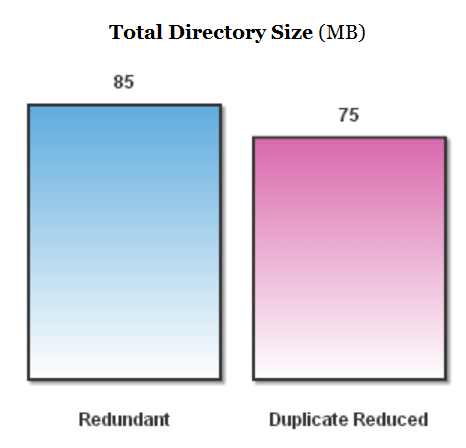
\includegraphics[width=2.5in]{smallaverage}
\caption{Average of 5 tests using different groups of sub 1MB images.}
\label{fig:smallaverage}
\end{figure}

\begin{figure}[htbp]
\centering
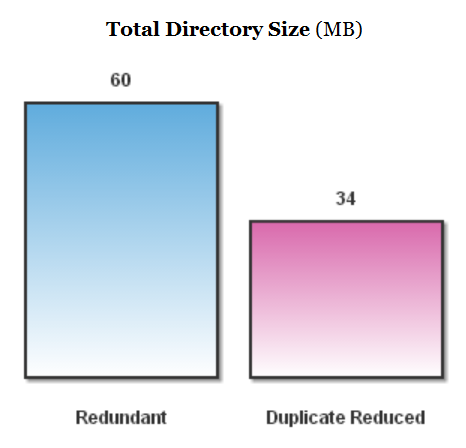
\includegraphics[width=2.5in]{largeaverage}
\caption{Average of 5 tests using different groups of greater than 1MB images.}
\label{fig:largeaverage}
\end{figure}

Last, and perhaps most importantly, accuracy for duplicate detection is how well the system worked when finding duplicates in a set of known files. After analyzing the results, the data was able to be broken down into three groups. These groups include small size photographs, large size photographs, and computer generated graphics. With both photographic groups, the accuracy was within the expected and acceptable range for locating duplicates. The system determined the expected outcome for each of 100 small photographic image files 82 times. It also determined the expected outcome for each of 100 large photographic image files 91 times. Many variables could have lead to the difference in correct detection between the two sets even though they contained the same images in different resolutions. After analyzing the results, the most probable cause of incorrect classification came from the loss of data involved with re-sizing the images to $16 \times 16$ pixels for deep analysis. This will be discussed in further detail when analyzing the computer generated graphics. Although the thumbnail size can be increased to improve accuracy, the processing time increases significantly due to the higher number of individual pixels needing analyzed.

Finally, the computer generated graphics provided completely unexpected results. On a set of 100 known images, only 33 were correctly identified. As mentioned previously, the process of generating the thumbnail for analysis causes a significant amount of data loss within the image. The computer graphics used all consisted of repetitive patterns of alternating black and white. As it turns out, the color profile is identical with each as each was developed to be half black and half white. If the image contained too much detail, when the thumbnail was generated the pattern is eliminated in many cases. This can be seen in Figure 
 
\section{Conclusion}
Coming soon.